\textbf{Исходный текст:} \\
    БГЯDSI!

\textbf{Публичный ключ $(e, n)$:} \\
    (1827821233260228957330462119381, 5791792681103248967722057525079)

\textbf{Приватный ключ $(d, n)$:} \\
    (2304676846327366406913727452413, 5791792681103248967722057525079)

\textbf{Зашифрованный текст:} \\
    3385608287236349261478244092696 2842962959242576787797687409723
    1026508350809114738769887424519 963820060395904968790397299828
    3789600647708532359425234605570 3104067190146191090063779640918
    1070021809437130113590398289664

Результаты работы программы представлены на рисунках~\ref{ris:encode-test-5}-\ref{ris:decode-test-5}.

\vspace{\baselineskip}
\begin{figure}[H]
\center{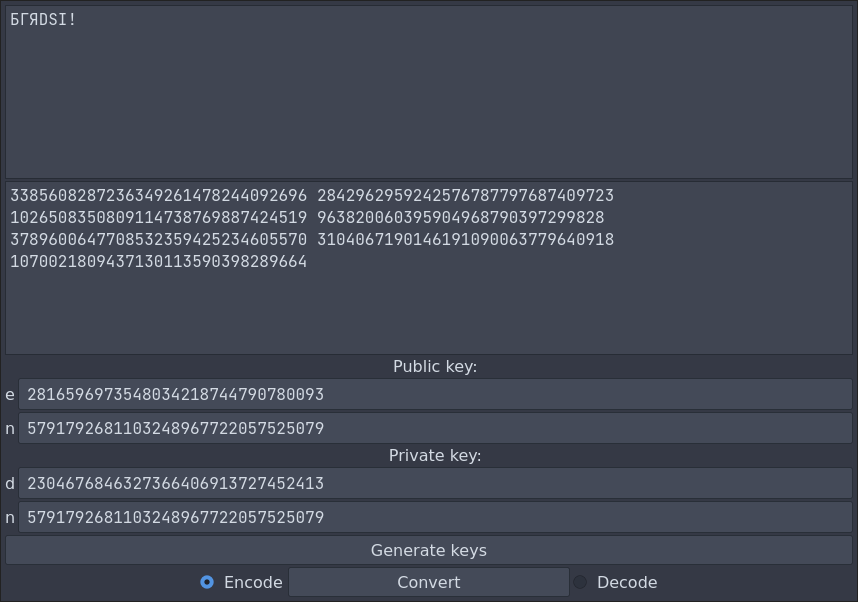
\includegraphics[width=0.8\linewidth]{figures/encode-test-5}}
    \caption{Шифрование}
\label{ris:encode-test-5}
\end{figure}

\vspace{\baselineskip}
\begin{figure}[H]
\center{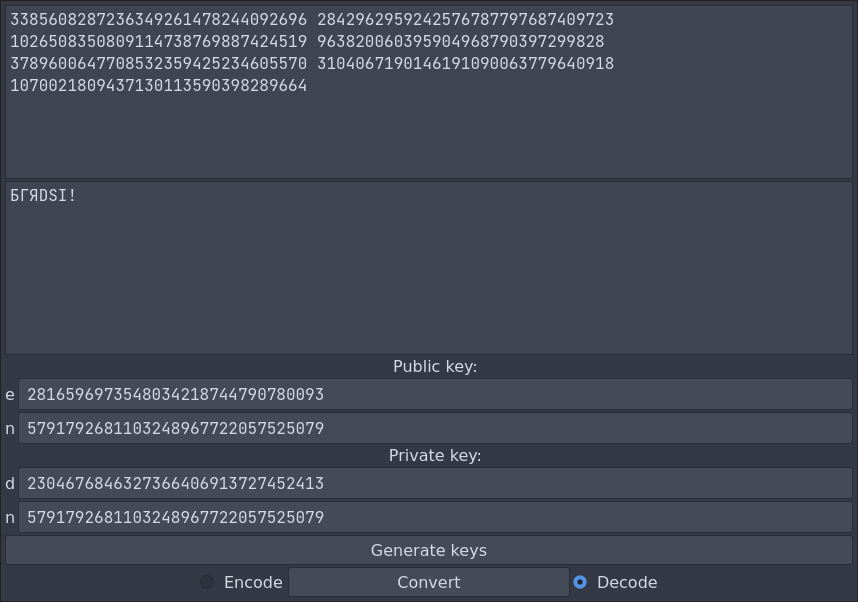
\includegraphics[width=0.8\linewidth]{figures/decode-test-5}}
    \caption{Расшифрование}
\label{ris:decode-test-5}
\end{figure}
